\documentclass[11pt]{article}
\usepackage[T1]{fontenc}
\usepackage[utf8]{inputenc}
\usepackage{mathpazo}
\usepackage{lmodern}\renewcommand{\rmdefault}{ppl}
\usepackage[margin=1in,headheight=14pt]{geometry}
\usepackage{xcolor}
\usepackage{amsmath,amssymb}
\usepackage{booktabs}
\usepackage{xltabular}
\usepackage{array}
\usepackage{enumitem}
\usepackage{fancyhdr}
\usepackage{titlesec}
\usepackage{listings}
\usepackage[most]{tcolorbox}
\usepackage{tikz}
\usetikzlibrary{arrows.meta,positioning,shapes.geometric}
\usepackage{xurl}
\usepackage[colorlinks=true,linkcolor=atlasblue,urlcolor=atlasblue]{hyperref}

\definecolor{atlasblue}{HTML}{1F4E79}
\definecolor{atlasteal}{HTML}{14776E}
\definecolor{atlasorange}{HTML}{B85C00}
\definecolor{atlasred}{HTML}{B3261E}
\definecolor{codebg}{HTML}{F3F4F6}
\definecolor{boxline}{HTML}{9AA3AD}
\definecolor{accentfill}{HTML}{E3EEF8}

\titleformat{\section}{\Large\bfseries\color{atlasblue}}{\thesection}{0.6em}{}
\titleformat{\subsection}{\large\bfseries\color{atlasblue}}{\thesubsection}{0.6em}{}
\titlespacing*{\section}{0pt}{18pt}{8pt}
\titlespacing*{\subsection}{0pt}{12pt}{5pt}

\pagestyle{fancy}
\fancyhf{}
\fancyhead[L]{\small\textcolor{atlasblue}{\textbf{Atlas v2}} -- 20-Hour Build Plan}
\fancyhead[R]{\small CodeRED: Orion}
\fancyfoot[C]{\small\thepage}
\renewcommand{\headrulewidth}{0.4pt}

\setlist{itemsep=2pt,topsep=4pt}
\setlength{\parindent}{0pt}
\setlength{\emergencystretch}{3em}
\setlength{\parskip}{5pt}
\renewcommand{\arraystretch}{1.25}

\newcommand{\code}[1]{\texttt{\detokenize{#1}}}
\newcommand{\verify}{\textbf{[VERIFY]}}
\newcommand{\cb}{$\square$\ }

\lstdefinestyle{sql}{
  language=SQL, basicstyle=\ttfamily\footnotesize, backgroundcolor=\color{codebg},
  keywordstyle=\color{atlasblue}\bfseries, commentstyle=\color{gray}\itshape,
  stringstyle=\color{atlasteal}, frame=single, rulecolor=\color{boxline},
  breaklines=true, columns=fullflexible, keepspaces=true, upquote=true,
  morekeywords={TIMESTAMPTZ,TEXT,BOOLEAN,BIGINT,NUMERIC,DOUBLE,PRECISION,MATERIALIZED,LATERAL,REFERENCES,INTERVAL,WITH,CROSS,HAVING,EXISTS}
}

\newtcolorbox{callout}[2][atlasblue]{colback=#1!4,colframe=#1,fonttitle=\bfseries,title=#2,arc=2pt,boxrule=0.8pt,left=6pt,right=6pt}

\newcolumntype{L}[1]{>{\raggedright\arraybackslash}p{#1}}
\newcolumntype{Y}{>{\raggedright\arraybackslash}X}

\begin{document}

%================ TITLE PAGE ================
\begin{titlepage}
\thispagestyle{empty}
\vspace*{3.2cm}
{\fontsize{46}{50}\selectfont\bfseries\color{atlasblue} Atlas\par}
\vspace{0.4cm}
{\LARGE Parametric flood protection for Houston\par}
\vspace{0.5cm}
{\large Fast cash in the first 72 hours, triggered by public gauge data, settled on Solana, priced on Tiger Data\par}
\vspace{0.8cm}
{\color{atlasblue}\rule{\linewidth}{0.8pt}}
\vspace{0.8cm}

{\large\bfseries 20-Hour Build Plan \textemdash{} Version 2\par}
\vspace{0.3cm}
CodeRED: Orion \quad | \quad Tracks: Overall, Pitch, Environment, Solana, Tiger Data, Vultr, GoDaddy\par
Team: 2 builders, JavaScript/TypeScript and Python only (no Rust)\par
As of October 10, 2026\par
\vspace{1cm}

\begin{callout}{The one-sentence pitch}
Maria rents in Meyerland. When Brays Bayou crosses flood stage, \$500 lands on her phone before the water goes down. That pays for a hotel, food and a missed shift in the first 72 hours, when nothing else pays.
\end{callout}

\vfill
{\small Assumptions behind this plan: a team of two, a 20-hour build inside a 24-hour clock, devnet only, no custom Solana program. Items marked \verify{} must be checked in Hours 0 to 1.5 (section~15).\par}
\end{titlepage}

\tableofcontents
\newpage

%================ 0 CHANGES ================
\section*{Changes from v1}
\addcontentsline{toc}{section}{Changes from v1}

v2 fixes eight demo-breaking bugs, rebuilds Person B's column so a simple version of every step works first and the upgrades come after, and adds hosting plus three more prize tracks. Everything not listed here is unchanged from v1.

{\small
\begin{xltabular}{\linewidth}{@{}r L{4.6cm} Y L{1.3cm}@{}}
\toprule
\# & v1 problem & v2 fix & Section \\
\midrule
\endhead
1 & Replay of Aug 20 to Sep 10 at 200x takes about 2.6 hours & Replay only the peak window (about 400 readings per gauge) in about 90 seconds; speed set by a config value & 6.5 \\
2 & Replay writes 2017 timestamps but policies start in 2026, so no policy is active and nothing pays & Replay shifts every timestamp to now (``Harvey happening today'') & 6.5 \\
3 & A second replay run fires no triggers and collides with the unique index, so Gate G3 fails & \code{run_id} on readings, events and payouts; every query scoped to one run; \code{POST /replay/reset} & 6.2, 6.4 \\
4 & Continuous aggregate mixes \code{usgs} and \code{replay}, materializes only every 3 days, and real-time aggregation is off by default & \code{source} and \code{run_id} in the GROUP BY, \code{materialized_only = false}; live replay chart reads the raw table & 6.3 \\
5 & No hosted website, which the rules require; oracles and Blinks also need a public URL & Vultr deploy from Hour 2.5, GoDaddy domain, HTTPS & 9.3 \\
6 & Devnet USDC faucet gives about 10 USDC per day, too little to fund the pool & Own SPL mint \code{aUSD}, created in pre-flight & 8.1 \\
7 & A judge-named bayou may not trigger in Harvey & 4 pre-checked gauges offered as buttons & 10 \\
8 & Legacy USGS WaterServices is being retired, with possible blackouts in late 2026 & Backfill and cache in Hour 1; never call USGS live on stage; plan for the new API & 6.1 \\
9 & Person B carries 7 risky integrations, and Gate G2 depends on Switchboard, the riskiest & Simple version of every step working end to end by Hour 5; each upgrade timeboxed to 1 hour and done after G2 & 5, 8 \\
10 & Pay-then-mint purchase can take payment and issue no policy & One atomic transaction: premium transfer plus mint, backend partially signs & 8.3 \\
11 & Policy burned on payout, erasing the visible proof & Metadata set to \code{status: paid}; burn only at expiry & 8.2 \\
12 & Pro-rata payouts are impossible when payouts go out one by one & Payouts batched per trigger wave with a pay factor & 7.4 \\
13 & Premiums counted twice (reserve and bond coupon) & Explicit waterfall & 7.3 \\
14 & Three real policies cannot show a catastrophe & Simulated book of 2,000 policies for aggregate numbers, clearly labelled & 7.5 \\
15 & Sales freeze had no data source & NWS alerts API & 7.6 \\
16 & Pitch heavy on jargon, only a 4-minute version & Story led by a person; 90-second and 4-minute scripts; payout shown on a phone & 1, 10 \\
17 & Only three prize tracks entered & Adds Environment, Best Pitch, Vultr and GoDaddy & 1.5 \\
18 & Frontend time sinks (Leaflet SSR, web3.js versions) & Version pins and setup rules written down & 3, 9.2 \\
\bottomrule
\end{xltabular}
}

%================ 1 PRODUCT ================
\section{Product summary and scope}

Atlas pays a fixed sum to every covered household near a Houston bayou gauge within minutes of that gauge crossing flood stage. No claim form, no adjuster.

\subsection{The pitch, led by a person}
\begin{quote}\itshape
Maria rents in Meyerland. When Brays Bayou crosses flood stage, \$500 lands on her phone before the water goes down. That pays for a hotel, food and a missed shift in the first 72 hours, when nothing else pays.
\end{quote}
Keep the technology out of the first 30 seconds. The stack goes in the Solana and Tiger Data write-ups and in Q\&A.

\subsection{The problem}
US flood insurance runs mostly through the federal program, which has a waiting period before cover starts and claims that take weeks or months. Many Houston renters and homeowners have no flood cover at all. In the first 72 hours people need cash for a hotel, a car, food and lost wages.

\subsection{What Atlas does}
Atlas sells a small policy tied to the nearest stream gauge. If that gauge crosses a set flood level during the term, the policyholder gets a fixed payout (for example \$500) automatically. Atlas does \emph{not} pay for property damage and does not replace flood insurance.

\subsection{How each sponsor technology is used}
{\small
\begin{xltabular}{\linewidth}{@{}L{2.8cm} Y@{}}
\toprule
Sponsor & Use \\
\midrule
Tiger Data & Gauge history and live readings as hypertables; continuous aggregates for charts and history; trigger detection; pricing and stress tests; compression; the replay engine; a simulated 2,000-policy book \\
Solana & \code{aUSD} test stablecoin; policies as non-transferable Token-2022 tokens with on-chain metadata; atomic purchase transaction; Squads multisig vault; payout bot; Memo evidence; catastrophe bond token. Optional: Switchboard feed, Squads spending limit, Blink \\
Vultr & Hosts the API, the replay feed, the Action endpoints and the dashboard over HTTPS \\
GoDaddy Registry & Domain for the hosted site \\
\bottomrule
\end{xltabular}
}

\subsection{Tracks entered}
\begin{itemize}
\item Best Overall (\$1,000)
\item Best Pitch/Demo (\$500)
\item Best Environment Hack (\$500): climate adaptation that protects a local community
\item Best Use of Solana
\item Best Use of Tiger Data
\item Best Use of Vultr
\item Best Domain Name from GoDaddy Registry
\end{itemize}
Open question: confirm Devpost allows one project in several tracks.

\subsection{In scope for the 20 hours}
\begin{itemize}
\item 6 to 10 Houston gauges with cached history and a live poller
\item Pricing with confidence bands; simulated book for aggregate numbers
\item Atomic purchase, payout on trigger, one payout per term
\item Catastrophe bond token with NAV
\item Harvey replay, time-shifted to now, about 90 seconds
\item Hosted dashboard: map, live chart, quote, pool, verify
\end{itemize}

\subsection{Out of scope}
Mainnet, real money, a custom Solana program, KYC, a mobile app, rainfall triggers, property-level flood modelling, and any claim to be a licensed insurance product.

%================ 2 ARCHITECTURE ================
\section{System architecture}

Every payout starts as a row in Tiger Data and ends as an \code{aUSD} transfer, with a Memo hash linking the two.

\begin{center}
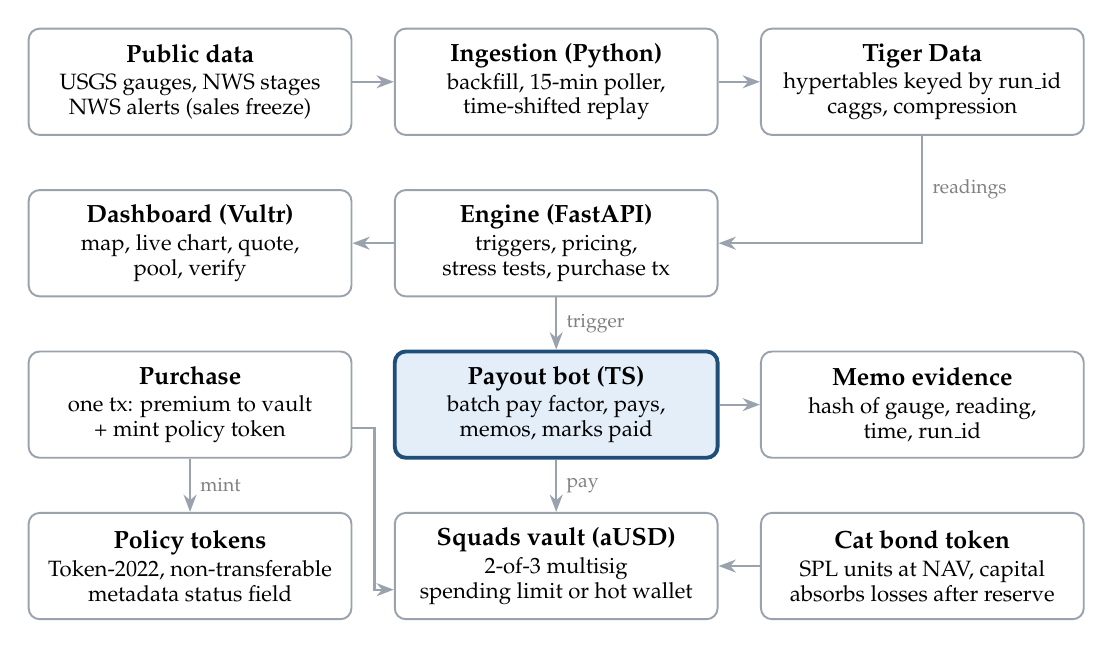
\begin{tikzpicture}[
  box/.style={draw=boxline, rounded corners=4pt, minimum width=4.1cm, minimum height=1.35cm, align=center, font=\small, line width=0.7pt},
  key/.style={box, draw=atlasblue, fill=accentfill, line width=1.4pt},
  arr/.style={-{Stealth[length=2.2mm]}, draw=boxline, line width=0.8pt},
  lbl/.style={font=\scriptsize\color{gray}}
]
\def\cx{4.65} \def\ry{2.05}
\node[box] (pub) at (0,0) {\textbf{Public data}\\[-1pt]{\footnotesize USGS gauges, NWS stages}\\[-2pt]{\footnotesize NWS alerts (sales freeze)}};
\node[box] (ing) at (\cx,0) {\textbf{Ingestion (Python)}\\[-1pt]{\footnotesize backfill, 15-min poller,}\\[-2pt]{\footnotesize time-shifted replay}};
\node[box] (tig) at (2*\cx,0) {\textbf{Tiger Data}\\[-1pt]{\footnotesize hypertables keyed by run\_id}\\[-2pt]{\footnotesize caggs, compression}};
\node[box] (dash) at (0,-\ry) {\textbf{Dashboard (Vultr)}\\[-1pt]{\footnotesize map, live chart, quote,}\\[-2pt]{\footnotesize pool, verify}};
\node[box] (eng) at (\cx,-\ry) {\textbf{Engine (FastAPI)}\\[-1pt]{\footnotesize triggers, pricing,}\\[-2pt]{\footnotesize stress tests, purchase tx}};
\node[box] (pur) at (0,-2*\ry) {\textbf{Purchase}\\[-1pt]{\footnotesize one tx: premium to vault}\\[-2pt]{\footnotesize + mint policy token}};
\node[key] (bot) at (\cx,-2*\ry) {\textbf{Payout bot (TS)}\\[-1pt]{\footnotesize batch pay factor, pays,}\\[-2pt]{\footnotesize memos, marks paid}};
\node[box] (memo) at (2*\cx,-2*\ry) {\textbf{Memo evidence}\\[-1pt]{\footnotesize hash of gauge, reading,}\\[-2pt]{\footnotesize time, run\_id}};
\node[box] (pol) at (0,-3*\ry) {\textbf{Policy tokens}\\[-1pt]{\footnotesize Token-2022, non-transferable}\\[-2pt]{\footnotesize metadata status field}};
\node[box] (vault) at (\cx,-3*\ry) {\textbf{Squads vault (aUSD)}\\[-1pt]{\footnotesize 2-of-3 multisig}\\[-2pt]{\footnotesize spending limit or hot wallet}};
\node[box] (bond) at (2*\cx,-3*\ry) {\textbf{Cat bond token}\\[-1pt]{\footnotesize SPL units at NAV, capital}\\[-2pt]{\footnotesize absorbs losses after reserve}};
\draw[arr] (pub) -- (ing);
\draw[arr] (ing) -- (tig);
\draw[arr] (tig.south) |- node[lbl, pos=0.25, right] {readings} (eng.east);
\draw[arr] (eng) -- (dash);
\draw[arr] (eng) -- node[lbl, right] {trigger} (bot);
\draw[arr] (bot) -- (memo);
\draw[arr] (bot) -- node[lbl, right] {pay} (vault);
\draw[arr] (bond) -- (vault);
\draw[arr] (pur) -- node[lbl, right] {mint} (pol);
\draw[arr] ([yshift=-3mm]pur.east) -- ++(0.28,0) |- ([yshift=-3mm]vault.west);
\end{tikzpicture}
\end{center}

The payout bot (highlighted) is the only component that moves money. Everything on Vultr is reachable over public HTTPS.

\subsection{Data flow for a single payout}
\begin{enumerate}
\item The poller (or the replay streamer) writes a reading into \code{gauge_readings} with its \code{source} and \code{run_id}.
\item The trigger query (6.4) finds gauges whose last two readings in that run are at or above \code{trigger_ft} with no open event in that run.
\item The engine writes a \code{trigger_events} row and computes the evidence hash.
\item The bot groups every gauge that triggered in the same wave and selects active, unpaid policies on them. It cross-checks each policy's on-chain metadata against Tiger before paying.
\item The bot computes the pay factor for the wave: \code{min(1, available / wave_total)} (7.4).
\item One transaction per policy: create the holder's token account if needed, transfer \code{aUSD} from the bot's float (or from the vault through the spending limit, if that upgrade ships), write the Memo.
\item The bot sets the policy's metadata field \code{status} to \code{paid}.
\item The payout is logged in \code{payouts} and appears on the pool page and the holder's phone.
\end{enumerate}
If Switchboard ships (8.8), step 3 also cranks the feed, and step 4 reads the on-chain value and checks it is fresh before paying.

%================ 3 PREFLIGHT ================
\section{Pre-flight checklist (first 30 minutes)}

Every item here removes a dependency on something outside your control before you write product code.

\textbf{Accounts and infrastructure}
\begin{itemize}[label=\cb]
\item Tiger Cloud service running; connection string tested from both laptops; free-tier limits noted. Local fallback: \code{timescale/timescaledb} Docker image.
\item Vultr instance up with HTTPS (Caddy is the quickest way to get a certificate); free credits claimed.
\item GoDaddy Registry domain registered and pointed at the Vultr IP.
\item Devnet RPC provider key (public devnet endpoints rate-limit hard).
\end{itemize}

\textbf{Chain setup (Person B)}
\begin{itemize}[label=\cb]
\item Devnet SOL in every wallet: 3 policyholders, 1 investor, the bot keypair, 3 multisig members. Use the web faucet early and from several sources.
\item Own SPL mint \code{aUSD} (6 decimals) created, and 1,000,000 \code{aUSD} minted to a treasury wallet. Do not depend on the Circle faucet: it gives about 10 USDC per day.
\item Phone wallet (Phantom) switched to Testnet Mode and funded.
\end{itemize}

\textbf{Code setup}
\begin{itemize}[label=\cb]
\item Monorepo: \code{/data}, \code{/engine}, \code{/chain}, \code{/web}, \code{/docs}, plus \code{.env.example}; secrets kept outside the repo.
\item Pin \code{@solana/web3.js@1.x}. Squads, \code{spl-token} and Switchboard are built on v1; do not install \code{@solana/kit}.
\item Node 20+, Python 3.11, Solana CLI on both laptops.
\end{itemize}

\textbf{Product}
\begin{itemize}[label=\cb]
\item Gauge shortlist drafted (6.1), with real USGS site numbers.
\item Track descriptions and judging criteria pasted into \code{/docs/criteria.md}.
\item API contract written to \code{/docs/api.md} (section 4.2).
\end{itemize}

%================ 4 ROLES ================
\section{Team roles and the API contract}

Person A owns every number; Person B owns every transaction and every pixel. The API contract written in Hour 1 lets B build the UI against mock JSON instead of waiting for A.

\subsection{Roles}
{\small
\begin{xltabular}{\linewidth}{@{}L{3.6cm} Y@{}}
\toprule
Role & Owns \\
\midrule
Person A: data and risk (Zeke) & Tiger schema, ingestion and cache, trigger logic, replay engine, pricing, simulated book, stress tests, bond maths, FastAPI read endpoints. Owns every number shown on stage. \\
Person B: chain and product & \code{aUSD}, policy mints, atomic purchase, Squads vault, payout bot, Memo evidence, bond token, dashboard, Vultr deploy and domain. Owns the live demo flow. Optional upgrades in 8.8. \\
Shared & Integration at each gate, pitch, Q\&A, recorded fallback video, Devpost write-up \\
\bottomrule
\end{xltabular}
}

\subsection{API contract (write to \texttt{/docs/api.md} in Hour 1)}
B serves mock JSON with these exact shapes from \code{/web/mocks} until A's endpoints are live. Only the shapes are fixed now; field names can be renamed together at Gate G1.

{\small
\begin{xltabular}{\linewidth}{@{}L{4.4cm} Y L{1.2cm}@{}}
\toprule
Endpoint & Returns & Owner \\
\midrule
\endhead
\code{GET /gauges} & \code{[{gauge_id, name, lat, lon, trigger_ft, latest_ft, status}]}, status is normal / near / triggered & A \\
\code{GET /gauges/{id}/}\allowbreak\code{series?run_id=} & \code{[{time, stage_ft}]} plus \code{trigger_ft} & A \\
\code{GET /quote?gauge=&payout=} & \code{{premium, p_payout, band: [p5, p95], waiting_days, sales_open, reason}} & A \\
\code{GET /pool} & \code{{reserve, bond_capital, nav_per_unit, premiums_in, payouts_out, coverage_outstanding, onchain, simulated}} & A \\
\code{GET /events?run_id=} & \code{[{time, gauge_id, reading_ft, evidence_hash, pay_factor, payouts: [{policy, tx_sig, memo_sig}]}]} & A, B fills tx fields \\
\code{GET /stress?scenario=harvey} & \code{{aggregate_loss, reserve_used, bond_used, prorata_cut, investor_loss_pct}} & A \\
\code{POST /replay/start}, \code{POST /replay/reset} & \code{{run_id}} & A \\
\code{GET /policies?owner=} & \code{[{policy_mint, gauge_id, payout, starts_at, ends_at, status}]} & B \\
\code{GET/POST}\allowbreak\ \code{/api/actions/buy?gauge=} & Action metadata, then a partially signed purchase transaction & B \\
\bottomrule
\end{xltabular}
}

%================ 5 TIMELINE ================
\section{Hour-by-hour timeline}

Gate G2 moves from Hour 7 to Hour 5 and needs no optional upgrade: one replay must pay one real devnet policy using a hot wallet and a Memo. Hour 0 is the start of hacking (1:00 pm CDT, Oct 10). The hard deadline is Hour 24, so the plan submits at Hour 19.5 and keeps 4.5 hours of slack. Spend that slack on sleep and rehearsal, not new scope.

\begin{center}
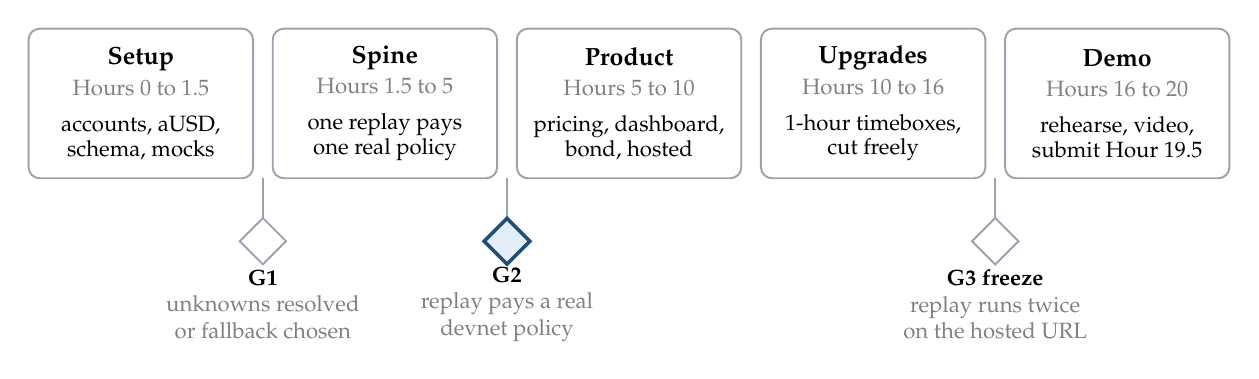
\begin{tikzpicture}[
  band/.style={draw=boxline, rounded corners=4pt, minimum width=2.85cm, minimum height=1.9cm, align=center, font=\small, line width=0.7pt},
  gmark/.style={diamond, draw=boxline, line width=0.7pt, minimum size=0.6cm, inner sep=0pt},
  keymark/.style={gmark, draw=atlasblue, fill=accentfill, line width=1.3pt},
  glbl/.style={align=center, font=\footnotesize}
]
\def\st{3.1}
\node[band] (b0) at (0,0) {\textbf{Setup}\\{\footnotesize\color{gray} Hours 0 to 1.5}\\[2pt]{\footnotesize accounts, aUSD,}\\[-2pt]{\footnotesize schema, mocks}};
\node[band] (b1) at (\st,0) {\textbf{Spine}\\{\footnotesize\color{gray} Hours 1.5 to 5}\\[2pt]{\footnotesize one replay pays}\\[-2pt]{\footnotesize one real policy}};
\node[band] (b2) at (2*\st,0) {\textbf{Product}\\{\footnotesize\color{gray} Hours 5 to 10}\\[2pt]{\footnotesize pricing, dashboard,}\\[-2pt]{\footnotesize bond, hosted}};
\node[band] (b3) at (3*\st,0) {\textbf{Upgrades}\\{\footnotesize\color{gray} Hours 10 to 16}\\[2pt]{\footnotesize 1-hour timeboxes,}\\[-2pt]{\footnotesize cut freely}};
\node[band] (b4) at (4*\st,0) {\textbf{Demo}\\{\footnotesize\color{gray} Hours 16 to 20}\\[2pt]{\footnotesize rehearse, video,}\\[-2pt]{\footnotesize submit Hour 19.5}};
\draw[draw=boxline, line width=0.7pt] (1.55,-0.95) -- (1.55,-1.45);
\node[gmark] at (1.55,-1.75) {};
\node[glbl] at (1.55,-2.55) {\textbf{G1}\\{\color{gray}unknowns resolved}\\{\color{gray}or fallback chosen}};
\draw[draw=boxline, line width=0.7pt] (4.65,-0.95) -- (4.65,-1.45);
\node[keymark] at (4.65,-1.75) {};
\node[glbl] at (4.65,-2.55) {\textbf{G2}\\{\color{gray}replay pays a real}\\{\color{gray}devnet policy}};
\draw[draw=boxline, line width=0.7pt] (10.85,-0.95) -- (10.85,-1.45);
\node[gmark] at (10.85,-1.75) {};
\node[glbl] at (10.85,-2.55) {\textbf{G3 freeze}\\{\color{gray}replay runs twice}\\{\color{gray}on the hosted URL}};
\end{tikzpicture}
\end{center}

\begin{callout}[atlasorange]{Rule for the whole build}
If a task blocks you for 45 minutes, say so out loud and switch to its fallback (section 12). An upgrade that misses its 1-hour timebox is dropped, not extended.
\end{callout}

{\small
\begin{xltabular}{\linewidth}{@{}L{1.5cm} Y Y@{}}
\toprule
Hours & Person A (data and risk) & Person B (chain and product) \\
\midrule
\endhead
0 to 1.5 & Confirm USGS access on both the legacy and new APIs; pick gauges with real site numbers; create schema with \code{run_id}; start writing raw JSON to disk & Pre-flight chain items (section 3); plain 2-of-3 Squads multisig; Token-2022 extension test script; mock JSON for every endpoint in 4.2 \\
\midrule
\multicolumn{3}{@{}l}{\textcolor{atlasteal}{\textbf{Gate G1 (Hour 1.5):}} every \verify{} item green or its fallback written in \code{/docs/decisions.md}} \\
\midrule
1.5 to 4 & Backfill the Harvey peak window and annual peaks into Tiger from the disk cache; live poller; continuous aggregates & Pre-create policy mints; atomic purchase transaction signed from a script; Vultr, HTTPS and domain live by Hour 2.5 \\
4 to 5 & Trigger query with guards; time-shifted replay streamer with \code{run_id} and reset & Simple payout bot: hot wallet pays \code{aUSD}, writes Memo, sets \code{status: paid} \\
\midrule
\multicolumn{3}{@{}p{\linewidth}@{}}{\textcolor{atlasteal}{\textbf{Gate G2 (Hour 5):}} a replay run triggers a gauge and a real devnet transaction pays a real policy. If not, cut scope now.} \\
\midrule
5 to 8 & Event frequency, premium, bootstrap band; simulated 2,000-policy book; waterfall; pay factor; real FastAPI endpoints & Dashboard against mocks: map, gauge chart, quote panel with wallet-adapter Buy button, pool page \\
8 to 10 & Harvey stress test; bond sizing; NWS alerts sales freeze & Bond token (deposit and mint units in one transaction); swap mocks for real API; deploy everything to Vultr \\
10 to 11 & \multicolumn{2}{L{11.2cm}}{Integration, eat, re-check every service; tag \code{v0.1}} \\
11 to 14 & Replay polish (about 90 seconds, map colours); \code{/docs/numbers.sql} & Upgrades, 1 hour each, in this order: Solana Pay QR or Blink; Squads spending limit; Switchboard feed. Then verify page and on-screen phone mirror. \\
14 to 16 & \multicolumn{2}{L{11.2cm}}{Staggered rest: A rests 14 to 15 while B polishes UI; B rests 15 to 16 while A runs the numbers audit} \\
\midrule
\multicolumn{3}{@{}p{\linewidth}@{}}{\textcolor{atlasteal}{\textbf{Gate G3 (Hour 16):}} feature freeze. The replay runs twice back to back, using reset, on the hosted URL, without touching code.} \\
\midrule
16 to 18 & Pitch slides with pricing and stress numbers; Q\&A drill & Two rehearsals each of the 90-second and 4-minute scripts; record the fallback video \\
18 to 19.5 & README, architecture diagram, setup steps & Devpost page, screenshots, track selection, on-chain address list \\
19.5 to 24 & \multicolumn{2}{L{11.2cm}}{Submitted. Sleep in shifts, then a final rehearsal before judging.} \\
\bottomrule
\end{xltabular}
}

%================ 6 DATA ================
\section{Data layer: Tiger Data}

Every row now carries \code{source} and \code{run_id}, the replay is shifted to the present, and nothing on stage depends on a live USGS call.

\subsection{Sources}
\begin{itemize}
\item \textbf{USGS (legacy WaterServices):} instantaneous stage and discharge, about every 15 minutes, plus annual peaks. USGS will retire it in Q1 2027 and warns of possible deliberate degradation and blackouts in the second half of 2026, which is now.
\item \textbf{USGS (new API, \code{api.waterdata.usgs.gov}):} check in Hour 0 which endpoints cover your gauges. Use it for the live poller if the legacy service is degraded.
\item \textbf{NWS flood stages:} action, minor, moderate and major stage per forecast point, used to set \code{trigger_ft}. \verify{} access path.
\item \textbf{NWS alerts (\code{api.weather.gov/alerts}):} active flood watches and warnings by point. Drives the sales freeze (7.6).
\item \textbf{Harris County Flood Warning System:} skip unless a documented API turns up in Hour 0.
\end{itemize}

\textbf{Cache rule:} every raw response is written to \code{/data/cache/} before parsing. Backfill and the replay read only from Tiger or the cache. Nothing on stage calls USGS.

\textbf{Gauge selection:} 6 to 10 gauges on major bayous (Buffalo, Brays, White Oak, Greens, Sims, Cypress Creek) with live data, at least 20 years of peaks, and data through Harvey. Use real site numbers. Mark the 4 that cross \code{trigger_ft} in the replay window; those are the demo buttons (section 10). Note any gauge that went offline during Harvey for the limitations section.

\subsection{Schema}
\begin{lstlisting}[style=sql]
-- Raw readings: one row per gauge, timestamp, source and run
CREATE TABLE gauge_readings (
  time          TIMESTAMPTZ NOT NULL,
  gauge_id      TEXT NOT NULL,
  stage_ft      DOUBLE PRECISION,
  discharge_cfs DOUBLE PRECISION,
  source        TEXT NOT NULL,                 -- 'usgs' | 'replay'
  run_id        TEXT NOT NULL DEFAULT 'live',
  rejected      BOOLEAN NOT NULL DEFAULT false, -- set by the data-quality guard
  ingested_at   TIMESTAMPTZ DEFAULT now()
);
SELECT create_hypertable('gauge_readings', by_range('time'));
CREATE UNIQUE INDEX ON gauge_readings (gauge_id, time, source, run_id);

CREATE TABLE gauges (
  gauge_id TEXT PRIMARY KEY, name TEXT, lat DOUBLE PRECISION, lon DOUBLE PRECISION,
  trigger_ft DOUBLE PRECISION, nws_flood_ft DOUBLE PRECISION,
  feed_pubkey TEXT, demo_ready BOOLEAN DEFAULT false
);

CREATE TABLE annual_peaks (
  gauge_id TEXT, water_year INT, peak_stage_ft DOUBLE PRECISION,
  peak_time TIMESTAMPTZ, PRIMARY KEY (gauge_id, water_year)
);

-- Mirror of on-chain policies; the bot cross-checks on-chain metadata before paying
CREATE TABLE policies (
  policy_mint TEXT PRIMARY KEY, owner TEXT NOT NULL,
  gauge_id TEXT REFERENCES gauges, payout_usd NUMERIC NOT NULL,
  premium_usd NUMERIC NOT NULL, starts_at TIMESTAMPTZ NOT NULL,
  ends_at TIMESTAMPTZ NOT NULL, status TEXT NOT NULL, -- active | paid | expired
  demo BOOLEAN NOT NULL DEFAULT false
);

-- Simulated book for aggregate numbers (7.5); never paid on-chain
CREATE TABLE sim_policies (
  sim_id BIGINT PRIMARY KEY, gauge_id TEXT REFERENCES gauges,
  payout_usd NUMERIC, premium_usd NUMERIC
);

CREATE TABLE trigger_events (
  time TIMESTAMPTZ NOT NULL, gauge_id TEXT NOT NULL,
  source TEXT NOT NULL, run_id TEXT NOT NULL, wave_id TEXT NOT NULL,
  reading_ft DOUBLE PRECISION, feed_value DOUBLE PRECISION, feed_slot BIGINT,
  evidence_hash TEXT
);
SELECT create_hypertable('trigger_events', by_range('time'));

CREATE TABLE payouts (
  time TIMESTAMPTZ NOT NULL, run_id TEXT NOT NULL, wave_id TEXT NOT NULL,
  policy_mint TEXT, owner TEXT, amount_usd NUMERIC, pay_factor NUMERIC,
  tx_sig TEXT, memo_sig TEXT
);
SELECT create_hypertable('payouts', by_range('time'));
\end{lstlisting}

\subsection{Continuous aggregates, compression, retention}
The aggregate now separates sources and runs, and shows rows that have not been materialized yet.
\begin{lstlisting}[style=sql]
CREATE MATERIALIZED VIEW gauge_hourly
WITH (timescaledb.continuous, timescaledb.materialized_only = false) AS
SELECT time_bucket('1 hour', time) AS bucket, gauge_id, source, run_id,
       max(stage_ft) AS max_stage, avg(stage_ft) AS avg_stage,
       max(discharge_cfs) AS max_q, count(*) AS n
FROM gauge_readings
WHERE NOT rejected
GROUP BY bucket, gauge_id, source, run_id;

SELECT add_continuous_aggregate_policy('gauge_hourly',
  start_offset => INTERVAL '3 days', end_offset => INTERVAL '15 minutes',
  schedule_interval => INTERVAL '15 minutes');

ALTER TABLE gauge_readings SET (
  timescaledb.compress,
  timescaledb.compress_segmentby = 'gauge_id, source',
  timescaledb.compress_orderby = 'time DESC');
SELECT add_compression_policy('gauge_readings', INTERVAL '7 days');
\end{lstlisting}
\begin{itemize}
\item History charts and the gauge page read \code{gauge_hourly}.
\item The live replay chart reads \code{gauge_readings} directly for the current \code{run_id}, so every new point appears at once.
\item Show the compression ratio from \code{hypertable_compression_stats} on a slide. Decades of backfill compress; replay rows are recent and stay uncompressed.
\end{itemize}

\subsection{Trigger query}
A gauge triggers when its last two accepted readings in this run are at or above \code{trigger_ft} and it has no event in this run within 72 hours.
\begin{lstlisting}[style=sql]
WITH last2 AS (
  SELECT g.gauge_id, g.trigger_ft, r.time, r.stage_ft
  FROM gauges g
  CROSS JOIN LATERAL (
    SELECT time, stage_ft FROM gauge_readings
    WHERE gauge_id = g.gauge_id AND source = $1 AND run_id = $2 AND NOT rejected
    ORDER BY time DESC LIMIT 2
  ) r
), crossed AS (
  SELECT gauge_id, max(time) AS time, max(stage_ft) AS stage_ft
  FROM last2
  GROUP BY gauge_id, trigger_ft
  HAVING count(*) = 2 AND min(stage_ft) >= trigger_ft
)
SELECT c.* FROM crossed c
WHERE NOT EXISTS (
  SELECT 1 FROM trigger_events e
  WHERE e.gauge_id = c.gauge_id AND e.run_id = $2
    AND e.time > c.time - INTERVAL '72 hours'
);
\end{lstlisting}

\textbf{Data-quality guard:} on insert, mark \code{rejected = true} when a reading jumps more than a set number of feet from the previous accepted reading within 15 minutes. Show the rejected count on the gauge page so judges see the guard working.

\textbf{Waves:} all gauges that cross in the same engine tick share one \code{wave_id}. The bot pays a wave together (7.4).

\subsection{Replay engine}
The replay plays only the flood peak, shifted so it starts now, in about 90 seconds.
\begin{itemize}
\item \textbf{Window:} from 48 hours before the first demo gauge crosses \code{trigger_ft} to 24 hours after the last peak. Expect roughly Aug 25 to Aug 30, 2017, about 430 readings per gauge. \verify{} the exact window from the stored data.
\item \textbf{Speed:} \code{REPLAY_SECONDS = 90} in config. Seconds per reading = \code{REPLAY_SECONDS / readings_in_window} (about 0.2 s).
\item \textbf{Time shift:} \code{replay_time = original_time + (wall_clock_at_start - window_start)}. The run starts at the present and runs forward, so a policy bought on stage a minute earlier is active when its gauge triggers.
\item \textbf{Runs:} \code{POST /replay/start} creates a new \code{run_id}. \code{POST /replay/reset} stops any run, deletes its replay rows and events, and sets demo policies back to \code{active} on-chain and in Tiger. Without the reset, the second rehearsal pays nothing because every demo policy is already \code{paid}.
\item \textbf{Feed endpoint:} \code{GET /replay/feed/{gauge_id}} returns the reading at the replay cursor for the current run. It is public on Vultr so a Switchboard feed (8.8) can read it.
\item \textbf{Evidence hash:} hash the value the bot acted on. Without Switchboard that is the Tiger reading; with Switchboard it is the on-chain feed value and slot. The verify page then always matches.
\end{itemize}

%================ 7 PRICING ================
\section{Pricing and capital model}

Pricing is unchanged from v1. v2 fixes how money flows: one explicit waterfall, payouts paid per wave with a pay factor, and a simulated book so the catastrophe numbers mean something.

\subsection{Event frequency}
For gauge $g$ with $T_g$ years of record and $N_g$ declustered events at or above its trigger level:
\[ \hat\lambda_g = \frac{N_g}{T_g} \]
Use annual peaks for the long record and instantaneous data to decluster recent years. Annual peaks count at most one event per year, so they slightly understate frequency; say so if asked. Stretch: fit a GEV to annual peaks with \code{scipy.stats.genextreme} and compare.

\subsection{Premium}
Each policy pays a fixed benefit $B$ at most once in a term of $t$ years. Treating events as Poisson:
\[ P(\text{payout}) = 1 - e^{-\hat\lambda_g t}, \qquad \mathbb{E}[L] = B\,\bigl(1 - e^{-\hat\lambda_g t}\bigr) \]
\[ \pi = \mathbb{E}[L]\,(1 + \theta) + c \cdot k \]
$\theta$ is the loading for expenses and uncertainty, $k$ the policy's share of required catastrophe capital, and $c$ the coupon rate paid to bond investors. Bootstrap the record 2,000 times and show the premium with a 5th to 95th percentile band.

\subsection{Waterfall (fixes double counting)}
Each premium is split once, in this order:
\begin{enumerate}
\item \textbf{Expenses:} a fixed share $e$ of $\pi$.
\item \textbf{Bond coupon:} $c \cdot k$, paid to bond holders over the term. This is the only source of bond yield.
\item \textbf{Reserve $R$:} the rest.
\end{enumerate}
Losses are absorbed in this order:
\begin{enumerate}
\item Reserve $R$.
\item Bond capital $C$.
\item Above $R + C$, payouts are cut by the pay factor (7.4). This is stated in the policy terms.
\end{enumerate}
\[ \text{NAV}_t = \frac{C - \text{losses absorbed}_t + \text{coupon accrued}_t}{\text{units outstanding}} \]

\subsection{Payouts per wave (fixes pro-rata)}
Paying gauges one at a time pays early gauges in full and leaves later ones with nothing. Instead, the bot pays each wave (6.4) together:
\[ f_w = \min\left(1,\ \frac{R_{\text{avail}} + C_{\text{avail}}}{B \cdot n_w}\right) \]
$n_w$ is the number of eligible policies in wave $w$. Every policy in the wave gets $f_w \cdot B$. A later wave in the same storm uses what is left; disclose that waves are paid in order.

\subsection{Simulated book (fixes the 3-policy problem)}
Three real policies cannot exhaust anything. The pool page shows two panels, each labelled:

{\small
\begin{xltabular}{\linewidth}{@{}L{2.6cm} Y L{3.2cm}@{}}
\toprule
Panel & Contents & Source \\
\midrule
On-chain (devnet) & 3 demo policies; reserve about 300 \code{aUSD}; bond capital 5,000 \code{aUSD}. Three \$500 payouts use the reserve, then the bond absorbs about 1,200 \code{aUSD} and NAV falls about 24\%. & Vault and mint balances \\
Simulated book & 2,000 policies in \code{sim_policies}, spread across gauges; Harvey aggregate loss, layer use, pro-rata cut, investor loss & Tiger, \code{/stress?}\allowbreak\code{scenario=harvey} \\
\bottomrule
\end{xltabular}
}
The on-chain numbers above are a sizing target; set the final figures from A's pricing so the bond absorbs a visible loss.

\subsection{Underwriting rules}
\begin{itemize}
\item Waiting period of 7 days between purchase and cover. Demo mode sets it to 0, and the demo says so aloud.
\item Sales freeze: \code{/quote} returns \code{sales_open: false} while \code{api.weather.gov/alerts} shows an active flood watch or warning at the gauge's location.
\item One policy per wallet per gauge, and a cap per wallet.
\end{itemize}

%================ 8 SOLANA ================
\section{Solana layer (Person B)}

The simple version (8.1 to 8.7) uses only token programs, Memo and a plain Squads multisig, and must work by Gate G2. Switchboard, spending limits and Blinks are 1-hour upgrades after it (8.8).

\subsection{Test stablecoin \texttt{aUSD}}
\begin{itemize}
\item A classic SPL Token mint, 6 decimals, created in pre-flight. Mint 1,000,000 to a treasury wallet and fund every demo wallet from it.
\item Policies use \textbf{Token-2022} and \code{aUSD} uses the \textbf{classic Token program}. Derive every associated token account with the right program ID; mixing them up is the most common silent failure.
\end{itemize}

\subsection{Policy tokens (Token-2022)}
Each policy is a mint with supply 1 and 0 decimals.
\begin{itemize}
\item \textbf{Extensions:} NonTransferable, MetadataPointer (pointing at itself), TokenMetadata. PermanentDelegate is added only if the Hour-0 test passes; it is used only for burning at expiry.
\item \textbf{Initialization order:} create the account sized for the fixed extensions but funded with lamports for the metadata as well, then initialize NonTransferable, PermanentDelegate and MetadataPointer, then \code{initializeMint}, then initialize metadata and add fields. A wrong order fails with unhelpful errors.
\item \textbf{Minimal metadata} (keeps the purchase transaction small): \code{policy_id}, \code{gauge_id}, \code{status}, \code{terms_hash}, plus a \code{uri} pointing to the full terms JSON on Vultr (payout, premium, start, end).
\item \textbf{Pre-created mints:} the backend keeps a pool of about 10 unminted policy mints per demo gauge, created in advance with metadata. This removes mint creation from the purchase transaction.
\item \textbf{Payout marks, not burns:} after payout the bot sets \code{status} to \code{paid}. ``PAID'' in the holder's wallet is the visible proof on stage. Burn only at expiry.
\item \textbf{Reset:} \code{/replay/reset} sets demo policies back to \code{active} (the backend holds update authority).
\end{itemize}

\subsection{Atomic purchase}
Payment and policy issue happen in one transaction, so a buyer can never pay without receiving a policy.
\begin{enumerate}
\item Client asks for a quote, then calls \code{POST /api/actions/buy?gauge=} with its wallet address.
\item Backend reserves one pre-created mint for 2 minutes (row lock in Tiger) and builds the transaction:
  \begin{enumerate}
  \item Create the buyer's Token-2022 account for the policy mint (idempotent).
  \item \code{transferChecked} of the premium in \code{aUSD} from buyer to the vault's token account.
  \item \code{mintTo} 1 policy token to the buyer.
  \item Remove the mint authority, so the policy can never be duplicated.
  \end{enumerate}
\item Backend partially signs as mint authority and returns the transaction; the buyer's wallet signs as fee payer and sends it.
\item On confirmation the backend writes the \code{policies} row. An unconfirmed reservation is released after 2 minutes.
\end{enumerate}
The same endpoint serves the Buy button, a Solana Pay QR and a Blink (8.8). Sign promptly: a blockhash expires in about a minute.

\subsection{Pool: Squads multisig}
\begin{itemize}
\item 2-of-3 Squads v4 multisig: both teammates plus a third key standing in for an independent trustee.
\item The vault is a PDA, so create its \code{aUSD} token account with \code{allowOwnerOffCurve = true}.
\item Set the time lock to about 60 seconds in demo mode. It applies to every proposal, including your own setup steps.
\item Simple version: one approved vault proposal moves a capped float (for example 2,000 \code{aUSD}) to the bot's hot wallet. Reserves stay in the vault.
\end{itemize}

\subsection{Payout bot (TypeScript)}
\begin{enumerate}
\item Poll \code{trigger_events} for a new \code{wave_id}.
\item For each eligible policy, cross-check on-chain: the holder still holds it, metadata \code{status} is \code{active}, \code{gauge_id} matches.
\item Compute the amount $f_w \cdot B$ (7.4).
\item One transaction per policy: create the holder's \code{aUSD} account (idempotent), \code{transferChecked} from the bot wallet, Memo with the evidence hash.
\item Set metadata \code{status} to \code{paid}, and write the \code{payouts} row.
\end{enumerate}
\textbf{Idempotency:} before paying, check \code{payouts} for the same policy and \code{run_id}. A restarted bot must never pay twice. Use a priority fee, confirm at \code{confirmed}, and retry with a fresh blockhash.

\subsection{Evidence anchoring}
\begin{itemize}
\item Memo text: \code{atlas:v1:<sha256>} over \code{gauge_id}, value acted on, time, \code{run_id}, \code{wave_id}, plus feed account and slot if Switchboard is live.
\item The verify page takes a payout signature, reads the Memo, recomputes the hash from \code{/events}, and shows the match with an Explorer link.
\item Say what this proves: an audit trail that the payout matches a recorded reading. It does not prove the reading is true; that is the oracle's job (8.8).
\end{itemize}

\subsection{Catastrophe bond token}
\begin{itemize}
\item Classic SPL mint; units are transferable.
\item Deposit is atomic, like purchase: the investor transfers \code{aUSD} to the vault and the backend partially signs \code{mintTo} for \code{deposit / NAV} units.
\item NAV is computed by the engine from vault balances and the waterfall (7.3), and shown on the pool page.
\item Redemption is the first thing cut. If asked, it is a multisig proposal after a notice period.
\end{itemize}

\subsection{Upgrades (after G2, 1 hour each, in this order)}
{\small
\begin{xltabular}{\linewidth}{@{}L{2.7cm} Y L{2.8cm}@{}}
\toprule
Upgrade & What to build & Drop it if \\
\midrule
Solana Pay QR or Blink & Same buy endpoint. Blink needs \code{actions.json} at the domain root and CORS headers on every Action route; test on dial.to. The phone's Phantom must be in Testnet Mode. A Solana Pay transaction-request QR is the more reliable fallback. & Not working on a phone in 1 hour \\
Squads spending limit & Config transaction adding a daily limit in \code{aUSD} for the bot key; the bot uses the spending-limit instruction instead of a hot-wallet float & Not paying through the limit in 1 hour \\
Switchboard on-demand feed & One feed per demo gauge: HTTP task on \code{/replay/feed/{gauge_id}} (public on Vultr), JSON parse. The bot cranks it on trigger, then pays only if the on-chain value is at or above \code{trigger_ft} and recent enough. & No on-chain value in 1 hour \\
\bottomrule
\end{xltabular}
}

%================ 9 BACKEND ================
\section{Backend, frontend and hosting}

Everything runs on one Vultr instance behind HTTPS on the GoDaddy domain from Hour 2.5, so the submission URL, the Action endpoints and the replay feed are public from early on.

\subsection{API (FastAPI)}
The full contract is in 4.2. Additions in v2:
\begin{itemize}
\item \code{POST /replay/reset} (6.5) and \code{run_id} on every series, event and payout read.
\item \code{GET /quote} returns \code{sales_open} and \code{reason} (7.6).
\item \code{GET /pool} returns separate \code{onchain} and \code{simulated} objects (7.5).
\item Buy and bond-deposit endpoints return partially signed transactions (8.3, 8.7).
\end{itemize}

\subsection{Frontend}
\textbf{Stack:} Next.js with Tailwind, Recharts and Leaflet, or Vite + React if Next.js fights you. Either way:
\begin{itemize}
\item Load the Leaflet map with \code{dynamic(() => import(...), { ssr: false })} in Next.js, or expect ``window is not defined''.
\item Put the wallet adapter in a \code{'use client'} provider component.
\item Build every page against \code{/web/mocks} first; switch to the real API at Hour 9.
\end{itemize}

{\small
\begin{xltabular}{\linewidth}{@{}L{2.4cm} Y@{}}
\toprule
Page & Shows \\
\midrule
Map & Houston gauges coloured normal, near, triggered; the replay clock; Start and Reset replay buttons (demo mode only) \\
Gauge & Stage over time with the trigger line, events marked, rejected-reading count, quote panel with band and Buy button \\
Pool & On-chain panel and simulated-book panel (7.5); bond NAV chart; payout feed with Explorer links \\
Verify & Paste a payout signature; see reading, Memo hash and match \\
Phone view & One wallet's policies with status and balance, large type, for mirroring on the projector \\
\bottomrule
\end{xltabular}
}

\subsection{Hosting}
\begin{itemize}
\item One Vultr instance runs FastAPI, the payout bot, the replay streamer and the built frontend, with Caddy for HTTPS.
\item The GoDaddy Registry domain points at it; \code{actions.json} is served at the domain root.
\item Processes run under \code{systemd} or \code{pm2} so they restart on crash. Check them all at Hour 10 and before judging.
\item Keep a local copy of the full stack runnable on a laptop as a fallback if the venue network or the instance fails.
\end{itemize}

%================ 10 DEMO ================
\section{Demo script}

The moment that wins is the payout landing on a phone everyone can see, at the instant the bayou line turns red. Both scripts are built around it. Expo-style table judging rarely gives 4 minutes, so the 90-second version is the default.

\textbf{Stage set-up:} the map on the laptop; the phone view (9.2) mirrored next to it; Start and Reset buttons visible; the fallback video open in another tab.

\subsection{90-second version}
{\small
\begin{xltabular}{\linewidth}{@{}L{2.4cm} Y@{}}
\toprule
Time & Beat \\
\midrule
0:00 to 0:15 & ``Maria rents in Meyerland. Federal flood claims take weeks. She needs money in the first 72 hours.'' \\
0:15 to 0:35 & Tap a demo gauge button (for example Brays Bayou). Show the quote: probability, premium, band. Buy on the phone; the policy appears in the wallet. \\
0:35 to 1:10 & Start the Harvey replay. Bayous rise, the map turns red, and the phone shows +\$500 and ``PAID''. \\
1:10 to 1:30 & Pool page: reserve used, the bond absorbs the rest. ``Priced from 30 years of gauge data in Tiger Data, settled on Solana in seconds.'' \\
\bottomrule
\end{xltabular}
}

\subsection{4-minute version}
{\small
\begin{xltabular}{\linewidth}{@{}L{2.4cm} Y@{}}
\toprule
Time & Beat \\
\midrule
0:00 to 0:30 & The gap, told through Maria. One sentence on Atlas. \\
0:30 to 1:15 & The judge picks one of the 4 demo gauge buttons. Quote with probability, premium, band and the history behind it. Buy on the phone; show the non-transferable policy in the wallet. Say: ``Waiting period is off in demo mode.'' \\
1:15 to 2:30 & Harvey replay, about 90 seconds. Map turns red, waves trigger, payouts land in three wallets, the phone shows PAID. Pool page: reserve exhausted, bond NAV drops. \\
2:30 to 3:00 & Verify one payout: Memo hash matches the recorded reading. \\
3:00 to 3:30 & Numbers: loss ratio, capital needed for a Harvey-scale event on the simulated book, Tiger compression ratio. \\
3:30 to 4:00 & Limitations in one breath (basis risk, licensing), then the close. \\
\bottomrule
\end{xltabular}
}

\begin{callout}[atlasred]{Demo rules}
\begin{itemize}[leftmargin=*]
\item Only offer the 4 gauges that cross their trigger in the replay window (6.1). Do not invite judges to name any bayou.
\item Press Reset before every judge group. Run one full replay 20 minutes before judging.
\item Pre-fund every wallet; keep phone Phantom in Testnet Mode with the screen-lock off.
\item Never debug in front of judges: switch to the fallback video within 15 seconds of anything breaking.
\end{itemize}
\end{callout}

%================ 11 QA ================
\section{Judge Q\&A preparation}

Three questions are new in v2 and are the ones a sharp judge will ask: who decides to pay, which numbers are real, and why the payout is fair in a big storm.

{\small
\begin{xltabular}{\linewidth}{@{}L{4.2cm} Y@{}}
\toprule
Question & Answer \\
\midrule
\endhead
Your bot decides to pay. What does the chain add? & Payment can't be separated from the policy: purchase is one atomic transaction. Every payout carries a Memo hash of the reading it acted on, so anyone can audit it. Pool solvency is public in real time. A Solana program that enforces the payout rule itself is the production step. \\
Which numbers are real? & On-chain panel: three real devnet policies and real vault balances. Simulated panel: a 2,000-policy book used for catastrophe numbers, labelled on screen. \\
What happens when the pool runs short in a big storm? & Reserve first, then the catastrophe bond, then every policy in a wave is cut by the same pay factor. Nobody is paid in full while others get nothing in the same wave. \\
What if the gauge triggers but my street stayed dry? & That is basis risk, the core trade-off of parametric cover. We trade precision for speed and keep payouts small and fixed for immediate needs. Rainfall and multi-gauge triggers are next. \\
Is this legal? & Selling insurance needs a licence, and the bond token is likely a security. Atlas is the engine an insurer, a city programme or a nonprofit would run; we would partner rather than sell directly. \\
Why blockchain? & Payout in seconds to anyone with a phone wallet, policies nobody can resell, evidence anyone can check, and a pool whose solvency is public. \\
Can you fake the oracle? & In this build the bot reads Tiger, and the replay is served by our server; we say so. With Switchboard, the live feed reads USGS directly and the bot checks the on-chain value and its freshness before paying. Production would use several sources. \\
Why not buy cover when a storm is coming? & A 7-day waiting period, and sales freeze while NWS has an active flood watch or warning at the gauge. \\
What if a gauge fails mid-flood? & It happens. Policy terms name a fallback: the nearest working gauge or a rainfall trigger. \\
How did you price it? & Declustered event frequency from decades of gauge history, Poisson payout probability, loading plus a capital charge, and a bootstrap confidence band. \\
Why mark the policy paid instead of burning it? & So the holder keeps visible proof of payment. It still pays once per term because the bot checks the status. It is burned at expiry. \\
How do you stop double payment if the bot crashes? & The bot checks for an existing payout for that policy and run before sending, and records every signature. \\
\bottomrule
\end{xltabular}
}

%================ 12 RISK ================
\section{Risk register, fallbacks and cut order}

The riskiest Solana pieces are now upgrades with their own 1-hour switch trigger, so no single SDK can block Gate G2.

{\small
\begin{xltabular}{\linewidth}{@{}L{3.6cm} L{1.5cm} L{3.4cm} Y@{}}
\toprule
Risk & Odds & Switch trigger & Fallback \\
\midrule
\endhead
USGS legacy service degraded or down & Medium & Any failed call in Hour 0 to 1 & New USGS API; otherwise disk cache only, live poller dropped and said so \\
Running out of time & High & Missed gate & Cut order below \\
Live demo failure on stage & Medium & Anything breaks & Fallback video, 15-second rule \\
Venue network or Vultr instance fails & Medium & Site unreachable & Local stack on a laptop, hotspot \\
Switchboard feed will not work on devnet & Medium & No on-chain value after its 1-hour box & Memo-only evidence; oracle presented as the production path \\
Squads spending limit fights back & Medium & Not paying through the limit after 1 hour & Hot-wallet float funded by one vault proposal \\
Blink will not render on the phone & Medium & Not working after 1 hour & Solana Pay QR, then the Buy button \\
Devnet congestion or airdrop limits & Medium & Failed airdrops or dropped transactions & Pre-funded wallets, own \code{aUSD}, priority fee and retry \\
Purchase transaction too large & Low to medium & Size error in Hour 1.5 to 4 & Fewer metadata fields; pre-created mints already remove the biggest part \\
Token-2022 extension combination fails & Low to medium & Hour 0 test & Drop PermanentDelegate; burn not needed for the demo \\
Replay too slow or out of order & Low & Rehearsal & Raise speed in config; pre-computed timeline with the same visuals \\
Tiger Cloud limits or outage & Low & Any blocking error & Local Docker TimescaleDB, same schema \\
\bottomrule
\end{xltabular}
}

\textbf{Cut order} (first cut first):
\begin{enumerate}
\item Bond redemption
\item GEV fit
\item Switchboard feed
\item Squads spending limit
\item Blink (keep the QR or Buy button)
\item Verify page
\item Bond deposit flow (seed bond capital by script instead)
\end{enumerate}
\textbf{Never cut:} the time-shifted replay with reset, the payout landing on the phone, the map turning red, the pool page, the hosted URL and the fallback video.

%================ 13 LIMITATIONS ================
\section{Limitations of the product}

State these briefly on stage and in full in the README; naming them first is more credible than being caught on them.

\subsection{Insurance design}
\begin{itemize}
\item \textbf{Basis risk:} payouts follow a gauge, not your property, so people can be paid without loss or flooded without payment.
\item \textbf{Fixed benefit:} Atlas pays for immediate needs, not property damage, and does not replace flood insurance.
\item \textbf{One payout per term:} back-to-back floods in one term pay once.
\item \textbf{Adverse selection:} waiting periods and sales freezes reduce, but do not remove, buying ahead of known risk.
\item \textbf{Waves paid in order:} a later wave in the same storm can receive a smaller pay factor than an earlier one.
\end{itemize}

\subsection{Data and oracle}
\begin{itemize}
\item \textbf{Gauge failure:} gauges can go offline in the largest floods, exactly when they matter.
\item \textbf{Provisional data:} real-time readings can be revised later; a payout on a provisional reading cannot be clawed back.
\item \textbf{Single source:} the live feed depends on one public provider, which USGS is itself migrating during this period.
\item \textbf{Replay trust:} the replay is served by the team's server, so it demonstrates the mechanism, not trustlessness.
\item \textbf{Off-chain decision:} without a custom program, the bot decides to pay. The Memo makes that decision auditable, not enforced.
\end{itemize}

\subsection{Pricing and capital}
\begin{itemize}
\item \textbf{Few extreme events:} a handful of major floods per gauge, so premiums carry wide uncertainty.
\item \textbf{Non-stationarity:} development, drainage projects and climate change shift flood frequency.
\item \textbf{Correlated losses:} one storm triggers most of the book at once; beyond reserve plus bond, payouts are cut.
\item \textbf{Simulated book:} catastrophe figures come from a simulated portfolio, not real sales.
\item \textbf{Bond investor risk:} holders can lose most of their principal in one event; pricing that properly needs far more modelling.
\end{itemize}

\subsection{Legal and regulatory}
\begin{itemize}
\item Selling policies would need a licensed insurer or an approved programme.
\item The bond token is likely a security.
\item Disclosure of basis risk and terms would be regulated.
\item Payouts depend on a stablecoin and its issuer.
\end{itemize}

\subsection{Users and adoption}
\begin{itemize}
\item Many people most exposed to floods hold no wallet or stablecoin; onboarding and cash-out are unsolved in this build.
\item A lost wallet means a lost policy, since policies are non-transferable.
\item People in a crisis may distrust an unfamiliar product.
\end{itemize}

\subsection{Hackathon build}
Devnet and test money only, a small gauge set, waiting period off in demo mode, custodial bot and mint keys, a hot-wallet float, and no audit of any code.

%================ 14 SUBMISSION ================
\section{Submission checklist}

Submit by Hour 19.5; the Devpost deadline is 1:00 pm CDT, Oct 11 (Hour 24).
\begin{itemize}[label=\cb]
\item \textbf{Hosted website URL} on the GoDaddy domain, working from a phone on mobile data.
\item Public repository with README: problem, architecture diagram, setup, how to run and reset the replay, limitations.
\item Every on-chain address listed: \code{aUSD} mint, an example policy mint, Squads multisig and vault, bond mint, bot key, feed accounts if any, sample payout and purchase transactions.
\item Demo video (2 to 3 minutes) of the full Harvey replay, with the phone visible.
\item Slides: problem through Maria, demo, pricing, stress test, Tiger Data usage, Solana usage, limitations, next steps.
\item Tracks selected: Overall, Pitch, Environment, Solana, Tiger Data, Vultr, GoDaddy. Each track's specific usage spelled out in the description.
\item \code{/docs/numbers.sql} reproduces every number on the slides.
\item Reset pressed and one full replay run 20 minutes before judging.
\end{itemize}

%================ 15 ASSUMPTIONS ================
\section{Unverified assumptions to check in Hours 0 to 1.5}

Each item needs a yes, or its fallback written into \code{/docs/decisions.md}, by Gate G1. Items v1 listed that v2 no longer depends on are removed: the Circle USDC faucet (replaced by \code{aUSD}), and Switchboard, spending limits and Blinks (now post-G2 upgrades).
\begin{itemize}[label=\cb]
\item USGS legacy instantaneous and peak endpoints still answer for the chosen gauges; which \code{api.waterdata.usgs.gov} endpoints cover them; rate limits; history depth.
\item NWS flood-stage access path for the chosen forecast points.
\item \code{api.weather.gov/alerts} returns flood watches and warnings by point.
\item Exact Harvey replay window and which 4 gauges cross \code{trigger_ft} in it, read from the stored data, not memory.
\item Token-2022 NonTransferable, MetadataPointer, TokenMetadata (and PermanentDelegate) on one mint via the JS library, with initialization in the order in 8.2.
\item The purchase transaction (8.3) fits under the 1,232-byte limit with the chosen metadata.
\item Squads v4 multisig, vault token account and time lock work on devnet with \code{@sqds/multisig} on \code{@solana/web3.js} 1.x.
\item Tiger Cloud free-tier limits, and whether the Tiger Data track requires Tiger Cloud specifically.
\item Devpost lets one project enter several tracks.
\item Phantom on the demo phone works in Testnet Mode and displays Token-2022 metadata.
\end{itemize}

\section*{Sources}
\addcontentsline{toc}{section}{Sources}
\begin{itemize}
\item USGS Water Data APIs (legacy WaterServices retirement in Q1 2027; possible degradation in late 2026): \url{https://www.usgs.gov/tools/usgs-water-data-apis}
\item USGS API decommission notice: \url{https://waterdata.usgs.gov/blog/api-decom-fall-2025/}
\item Circle testnet faucet (devnet USDC limits): \url{https://developers.circle.com/w3s/docs/developer-console-faucet}
\item CodeRED: Orion on Devpost (tracks, rules, deadline): \url{https://codered-orion-ccs.devpost.com/}
\end{itemize}

\end{document}
